\subsection{Qwen3-4B: four-round graph comparisons}
\label{app:qwen4b-four-round}

Both Qwen3-4B policies comprise five paired blocks and four rounds,
evaluated greedily on 2,000 ID and 1,000 OOD questions.
Table~\ref{tab:qwen4b-endpoints} reports endpoint accuracy and target incidence.
Unaudited OOD accuracy contrasts
at rounds two and three are $0.0308\pm0.0243$ and $0.0388\pm0.0233$,
but this intermediate advantage does not persist at round four.
These comparisons are not adjusted for multiplicity and do not constitute
a best-checkpoint analysis.

\begin{table}[H]
\caption{Qwen3-4B round-one matching, shared across both four-round policies and the one-step reuse. $N^+/N^-$ exclude truncated answers. Both arms have identical prompt and correct-response IDs, 48/16 correct/error quotas, and exact per-prompt supervised response lengths. Later checkpoint-dependent pools are not jointly matched.}
\label{tab:qwen4b-matching}
\centering\small\setlength{\tabcolsep}{3pt}
\begin{tabular}{@{}lllllll@{}}
\toprule
Block & $N^+/N^-$ & Cut & TPR/FPR & Yield & Target hits $R/S$ & Controls\\
\midrule
b00 & 10326/6049 & 9 & 0.004648/0.002645 & 0.003908 & 10/16 & pass\\
b01 & 10323/6054 & 7 & 0.004650/0.002643 & 0.003908 & 10/16 & pass\\
b02 & 10360/6014 & 10 & 0.004633/0.002660 & 0.003909 & 9/16 & pass\\
b03 & 10370/6009 & 5 & 0.004629/0.002663 & 0.003907 & 9/16 & pass\\
b04 & 10325/6050 & 9 & 0.004649/0.002645 & 0.003908 & 9/16 & pass\\
\bottomrule
\end{tabular}
\end{table}

\begin{table}[H]
\caption{Qwen3-4B graph endpoints after four rounds. Target rates count nonshortest answers among all evaluated questions. Paired $S-R$ differences are within policy, with descriptive 95\% block-$t$ half-widths over five blocks. Same-arm audit-change intervals appear in Table~\ref{tab:audit-results}.}
\label{tab:qwen4b-endpoints}
\centering\small\setlength{\tabcolsep}{3pt}
\begin{tabular}{@{}lllllll@{}}
\toprule
Split & Policy & Base & Pass@1 $R/S$ & $S-R$ Pass@1 & Target $R/S$ & $S-R$ target\\
\midrule
ID & None & 0.6125 & 0.7309/0.7339 & $0.0030\pm0.0968$ & 0.1026/0.1491 & $0.0465\pm0.1489$\\
ID & B=16 & 0.6100 & 0.7180/0.7273 & $0.0093\pm0.0745$ & 0.1375/0.1614 & $0.0239\pm0.0328$\\
OOD & None & 0.3970 & 0.4988/0.4982 & $-0.0006\pm0.0991$ & 0.1618/0.2644 & $0.1026\pm0.2015$\\
OOD & B=16 & 0.3960 & 0.4750/0.4850 & $0.0100\pm0.0741$ & 0.2060/0.2424 & $0.0364\pm0.0528$\\
\bottomrule
\end{tabular}
\end{table}


The identical round-one certificates confirm shared prompt/correct-response IDs,
$48/16$ correct/error counts, and exact response-token matching.
$R$ selects 9--10 nonshortest errors, versus 16 in $S$.
Audited training rows and weights agree with the reported
selection counts and effective sample sizes. Later pools are not jointly rate-matched.
Generation uses temperature $1.3$, top-$p=1$, and a mixed stopping schedule: block
\texttt{b00} uses no repetition stop throughout; \texttt{b01} introduces
it at round four, and \texttt{b02}--\texttt{b04} use it in later-round
generation throughout. The two arms share each block-round setting.
Their imported round-one pools were generated without this stop rule.
Thus the study is not a replication under one uniform generation profile.

Both policies improve in mean.
Same-arm audit error changes are positive in mean
(Table~\ref{tab:audit-results}). Each audited arm spends 64
queries per block, averaging 54.4/55.0 $R/S$ updates versus 64 unaudited.
These descriptive contrasts combine changes in data, weighting,
and optimizer effort.

Tables~\ref{tab:qwen4b-rounds} and~\ref{tab:qwen4b-blocks} report all four
rounds and all five endpoint blocks, rather than a selected checkpoint.
Table~\ref{tab:qwen4b-audit-change} gives accuracy changes with their
paired intervals, complementing the error changes in
Table~\ref{tab:audit-results}. Table~\ref{tab:qwen4b-audit} reports each
round's projection, retained volume, positive-weight coverage, ESS, and
TPRs. Retained-row TPR equals pre-audit TPR because audit deletion
preserves all 48 correct rows; positive-weight TPR can be smaller.
Rates use each round's original nontruncated-pool denominator and are
averages of block-level ratios, not ratios of pooled counts.
Table~\ref{tab:qwen4b-training} complements these readouts with per-round
parameter-change norms and training losses for the completed comparisons.
These quantities describe the training objective, not held-out accuracy;
losses under different weighting policies are not directly comparable.

\begin{table}[H]
\caption{Qwen3-4B four-round graph trajectories: means $\pm$ pointwise descriptive 95\% block-$t$ half-widths over five blocks. Target incidence counts nonshortest answers among all evaluated questions.}
\label{tab:qwen4b-rounds}
\centering\small\setlength{\tabcolsep}{3pt}
\begin{tabular}{@{}lllllllll@{}}
\toprule
Split & Policy & Round & Pass@1 $R$ & Pass@1 $S$ & Pass@1 $S-R$ & Target $R$ & Target $S$ & Target $S-R$\\
\midrule
ID & Base, none & 0 & 0.613 & 0.613 & --- & 0.215 & 0.215 & ---\\
ID & None & 1 & $0.614\pm0.032$ & $0.607\pm0.012$ & $-0.007\pm0.028$ & $0.215\pm0.029$ & $0.230\pm0.011$ & $0.015\pm0.030$\\
ID & None & 2 & $0.634\pm0.033$ & $0.650\pm0.034$ & $0.016\pm0.034$ & $0.196\pm0.035$ & $0.190\pm0.042$ & $-0.007\pm0.046$\\
ID & None & 3 & $0.680\pm0.022$ & $0.703\pm0.030$ & $0.023\pm0.039$ & $0.138\pm0.053$ & $0.155\pm0.053$ & $0.017\pm0.090$\\
ID & None & 4 & $0.731\pm0.056$ & $0.734\pm0.067$ & $0.003\pm0.097$ & $0.103\pm0.094$ & $0.149\pm0.076$ & $0.046\pm0.149$\\
ID & Base, B=16 & 0 & 0.610 & 0.610 & --- & 0.220 & 0.220 & ---\\
ID & B=16 & 1 & $0.622\pm0.025$ & $0.622\pm0.044$ & $0.000\pm0.036$ & $0.205\pm0.016$ & $0.213\pm0.048$ & $0.007\pm0.047$\\
ID & B=16 & 2 & $0.654\pm0.040$ & $0.663\pm0.071$ & $0.009\pm0.062$ & $0.179\pm0.047$ & $0.177\pm0.071$ & $-0.003\pm0.092$\\
ID & B=16 & 3 & $0.698\pm0.042$ & $0.714\pm0.084$ & $0.016\pm0.060$ & $0.143\pm0.042$ & $0.143\pm0.078$ & $-0.000\pm0.065$\\
ID & B=16 & 4 & $0.718\pm0.068$ & $0.727\pm0.072$ & $0.009\pm0.075$ & $0.138\pm0.068$ & $0.161\pm0.054$ & $0.024\pm0.033$\\
OOD & Base, none & 0 & 0.397 & 0.397 & --- & 0.260 & 0.260 & ---\\
OOD & None & 1 & $0.394\pm0.014$ & $0.392\pm0.011$ & $-0.002\pm0.022$ & $0.258\pm0.016$ & $0.285\pm0.018$ & $0.027\pm0.022$\\
OOD & None & 2 & $0.398\pm0.023$ & $0.429\pm0.027$ & $0.031\pm0.024$ & $0.250\pm0.029$ & $0.257\pm0.038$ & $0.006\pm0.046$\\
OOD & None & 3 & $0.432\pm0.019$ & $0.471\pm0.025$ & $0.039\pm0.023$ & $0.191\pm0.074$ & $0.253\pm0.047$ & $0.062\pm0.098$\\
OOD & None & 4 & $0.499\pm0.049$ & $0.498\pm0.062$ & $-0.001\pm0.099$ & $0.162\pm0.129$ & $0.264\pm0.084$ & $0.103\pm0.202$\\
OOD & Base, B=16 & 0 & 0.396 & 0.396 & --- & 0.260 & 0.260 & ---\\
OOD & B=16 & 1 & $0.399\pm0.031$ & $0.399\pm0.034$ & $-0.000\pm0.028$ & $0.246\pm0.010$ & $0.259\pm0.034$ & $0.013\pm0.040$\\
OOD & B=16 & 2 & $0.420\pm0.037$ & $0.429\pm0.058$ & $0.008\pm0.054$ & $0.236\pm0.048$ & $0.230\pm0.057$ & $-0.007\pm0.091$\\
OOD & B=16 & 3 & $0.459\pm0.029$ & $0.478\pm0.082$ & $0.019\pm0.064$ & $0.207\pm0.055$ & $0.205\pm0.066$ & $-0.002\pm0.076$\\
OOD & B=16 & 4 & $0.475\pm0.079$ & $0.485\pm0.048$ & $0.010\pm0.074$ & $0.206\pm0.058$ & $0.242\pm0.033$ & $0.036\pm0.053$\\
\bottomrule
\end{tabular}
\end{table}

\begin{table}[H]
\caption{Qwen3-4B round-four graph endpoints by paired block. Slash-separated entries are $R/S$ values, not ratios. All five blocks are retained, including unfavorable audit changes.}
\label{tab:qwen4b-blocks}
\centering\small\setlength{\tabcolsep}{3pt}
\begin{tabular}{@{}llllll@{}}
\toprule
Policy & Block & ID Pass@1 & OOD Pass@1 & ID target & OOD target\\
\midrule
None & b00 & 0.7115/0.6750 & 0.5030/0.4470 & 0.0325/0.1935 & 0.0480/0.3200\\
None & b01 & 0.6615/0.7710 & 0.4320/0.5490 & 0.2300/0.1100 & 0.3290/0.1910\\
None & b02 & 0.7740/0.6740 & 0.5340/0.4430 & 0.0690/0.2345 & 0.1190/0.3500\\
None & b03 & 0.7570/0.7700 & 0.5050/0.5150 & 0.1050/0.1055 & 0.1720/0.2280\\
None & b04 & 0.7505/0.7795 & 0.5200/0.5370 & 0.0765/0.1020 & 0.1410/0.2330\\
B=16 & b00 & 0.6295/0.7200 & 0.3920/0.4790 & 0.2045/0.1860 & 0.2290/0.2670\\
B=16 & b01 & 0.7250/0.7240 & 0.4420/0.4960 & 0.1205/0.1350 & 0.1920/0.1990\\
B=16 & b02 & 0.7520/0.7850 & 0.5250/0.5260 & 0.0940/0.1365 & 0.1670/0.2480\\
B=16 & b03 & 0.7115/0.6370 & 0.4650/0.4230 & 0.1855/0.2255 & 0.2760/0.2580\\
B=16 & b04 & 0.7720/0.7705 & 0.5510/0.5010 & 0.0830/0.1240 & 0.1660/0.2400\\
\bottomrule
\end{tabular}
\end{table}

\begin{table}[H]
\caption{Qwen3-4B same-arm audited-minus-unaudited accuracy changes at round four (positive favors auditing), with paired 95\% block-$t$ half-widths. Unaudited arms each take 64 steps; auditing also changes retained data, weights, and optimizer effort.}
\label{tab:qwen4b-audit-change}
\centering\small\setlength{\tabcolsep}{3pt}
\begin{tabular}{@{}lllll@{}}
\toprule
Arm & Queries & Audited steps: mean [range] & ID accuracy change & OOD accuracy change\\
\midrule
R & 64 & 54.4 [49--61] & $-0.0129\pm0.0706$ & $-0.0238\pm0.0687$\\
S & 64 & 55.0 [52--57] & $-0.0066\pm0.1147$ & $-0.0132\pm0.0869$\\
\bottomrule
\end{tabular}
\end{table}

\begin{table}[H]
\caption{Qwen3-4B graph update and audit readouts, means over five blocks. $K\prime$ counts retained rows, $n^+$ positive-weight rows, and ESS is verified from audited weights. TPRs are percentages on each round-specific original nontruncated pool: pre-audit $48/N^+$ and positive-weight correct count divided by $N^+$. All 48 correct rows survive deletion, so retained post-audit TPR equals pre-audit TPR. The projection uses the fixed initial reference gradient, not measured task risk.}
\label{tab:qwen4b-audit}
\centering\small\setlength{\tabcolsep}{3pt}
\begin{tabular}{@{}llllllllll@{}}
\toprule
Round & Policy & Arm & $h^T\Delta\theta_t$ & Steps & $K\prime$ & $n^+$ & ESS & Pre TPR (\%) & Positive TPR (\%)\\
\midrule
1 & None & R & $-0.1487$ & 16.0 & 64.0 & 64.0 & 64.00 & 0.4642 & 0.4642\\
1 & None & S & $-0.1479$ & 16.0 & 64.0 & 64.0 & 64.00 & 0.4642 & 0.4642\\
1 & B=16 & R & $-0.0707$ & 13.2 & 60.0 & 50.6 & 40.33 & 0.4642 & 0.3984\\
1 & B=16 & S & $-0.0918$ & 13.2 & 60.0 & 50.6 & 40.33 & 0.4642 & 0.3984\\
2 & None & R & $-0.0985$ & 16.0 & 64.0 & 64.0 & 64.00 & 0.4657 & 0.4657\\
2 & None & S & $-0.0902$ & 16.0 & 64.0 & 64.0 & 64.00 & 0.4733 & 0.4733\\
2 & B=16 & R & $-0.1181$ & 14.8 & 61.0 & 57.0 & 48.83 & 0.4589 & 0.4293\\
2 & B=16 & S & $-0.1208$ & 13.6 & 60.0 & 52.6 & 43.83 & 0.4663 & 0.4166\\
3 & None & R & $-0.0697$ & 16.0 & 64.0 & 64.0 & 64.00 & 0.5134 & 0.5134\\
3 & None & S & $-0.0651$ & 16.0 & 64.0 & 64.0 & 64.00 & 0.4895 & 0.4895\\
3 & B=16 & R & $-0.0819$ & 12.4 & 59.4 & 48.0 & 37.98 & 0.4684 & 0.3829\\
3 & B=16 & S & $-0.0836$ & 12.4 & 59.4 & 49.0 & 39.39 & 0.4698 & 0.3876\\
4 & None & R & $-0.0524$ & 16.0 & 64.0 & 64.0 & 64.00 & 0.5735 & 0.5735\\
4 & None & S & $-0.0323$ & 16.0 & 64.0 & 64.0 & 64.00 & 0.5305 & 0.5305\\
4 & B=16 & R & $-0.0444$ & 14.0 & 60.2 & 55.4 & 44.71 & 0.4523 & 0.4173\\
4 & B=16 & S & $-0.0488$ & 15.8 & 61.2 & 61.2 & 50.03 & 0.4546 & 0.4546\\
\bottomrule
\end{tabular}
\end{table}

\begin{table}[H]
\caption{Qwen3-4B four-round training diagnostics, means over five blocks per arm and policy. $\Delta\theta_t$ is the parameter change within round $t$; $h$ is fixed at initialization. Norms are not cumulative displacement norms, and loss is the policy-specific weighted training objective. Neither projection nor training loss is held-out task accuracy.}
\label{tab:qwen4b-training}
\centering\small\setlength{\tabcolsep}{4pt}
\begin{tabular}{@{}lllrrr@{}}
\toprule
Round & Audit & Arm & $h^T\Delta\theta_t$ & $\|\Delta\theta_t\|_2$ & Loss\\
\midrule
1 & None & R & $-0.1487$ & 1.5161 & 0.0309\\
1 & None & S & $-0.1479$ & 1.5474 & 0.0364\\
1 & B=16 & R & $-0.0707$ & 1.2888 & 0.0309\\
1 & B=16 & S & $-0.0918$ & 1.3315 & 0.0332\\
2 & None & R & $-0.0985$ & 1.6279 & 0.0415\\
2 & None & S & $-0.0902$ & 1.6084 & 0.0411\\
2 & B=16 & R & $-0.1181$ & 1.5290 & 0.0308\\
2 & B=16 & S & $-0.1208$ & 1.4442 & 0.0311\\
3 & None & R & $-0.0697$ & 1.5263 & 0.0714\\
3 & None & S & $-0.0651$ & 1.5377 & 0.0643\\
3 & B=16 & R & $-0.0819$ & 1.3484 & 0.0353\\
3 & B=16 & S & $-0.0836$ & 1.3693 & 0.0304\\
4 & None & R & $-0.0524$ & 1.5233 & 0.3888\\
4 & None & S & $-0.0323$ & 1.5071 & 0.0719\\
4 & B=16 & R & $-0.0444$ & 1.3811 & 0.0704\\
4 & B=16 & S & $-0.0488$ & 1.5224 & 0.0426\\
\bottomrule
\end{tabular}
\end{table}


\paragraph{Validation scope.}
Accuracy and target incidence are reconstructed from 82 checkpoint--split
count records per policy, with all 40 training completions per policy checked.
All 123,000 audited held-out responses are independently rejudged, including
truncated answers in the evaluation denominators. Audit queries, retained
volume, positive-weight counts, and ESS agree with the training records.
Unaudited validation remains count-based because answers are unavailable.
Audited checkpoints are not reloaded; missing shared initialization and
reference tensors preclude independent gradient recomputation.
The 81,920 shared round-one candidate responses are also independently
rejudged; eligible-pool counts agree with the matching certificates.
Exact-length eligibility is reported from those certificates rather than
independently retokenized.

\begin{figure}[H]
\centering
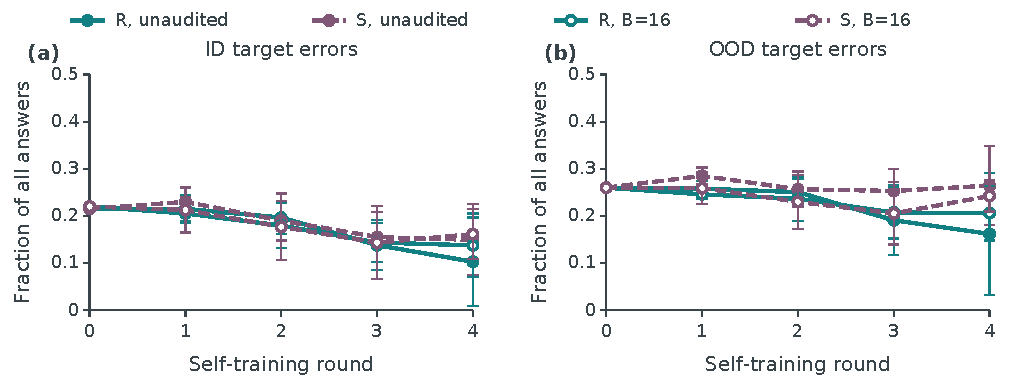
\includegraphics[width=0.8\linewidth]{figures/qwen4b_multiround/qwen4b_target_errors.pdf}
\caption{Qwen3-4B nonshortest-error incidence among all evaluated answers.
Unaudited $R/S$ endpoints are $0.1026/0.1491$ ID and $0.1618/0.2644$ OOD;
audited endpoints are $0.1375/0.1614$ and $0.2060/0.2424$.
Paired contrasts appear in Table~\ref{tab:qwen4b-endpoints}.
Bars are pointwise block-$t$ intervals
over five blocks.}
\label{fig:qwen4b-target-errors}
\end{figure}

\begingroup
\let\figure\RSIappendixfigure
\let\endfigure\RSIendappendixfigure
\subsubsection{Original four-round Qwen3-4B figures}
\label{app:qwen4b-raw-figures}

Figures~\ref{fig:qwen4b-raw-unaudited}--\ref{fig:qwen4b-raw-comparison-difficulty}
present the Qwen3-4B trajectories in the same six groups as
Appendix~\ref{app:qwen-raw-figures}: unaudited, audited, and joint
comparisons, each with aggregate and difficulty-stratified views.
The separate-policy plots are original exports; the joint views are
generated from the same checkpoint records with the same plotting method.
They complement Figure~\ref{fig:graph-four-round}(c--d) and
Table~\ref{tab:qwen4b-endpoints}, not additional experiments.
All use five paired blocks and fixed sets of 2,000 ID or 1,000 OOD
questions. Error bars are pointwise, descriptive 95\% block-$t$ intervals.

\begin{figure}[H]
\centering
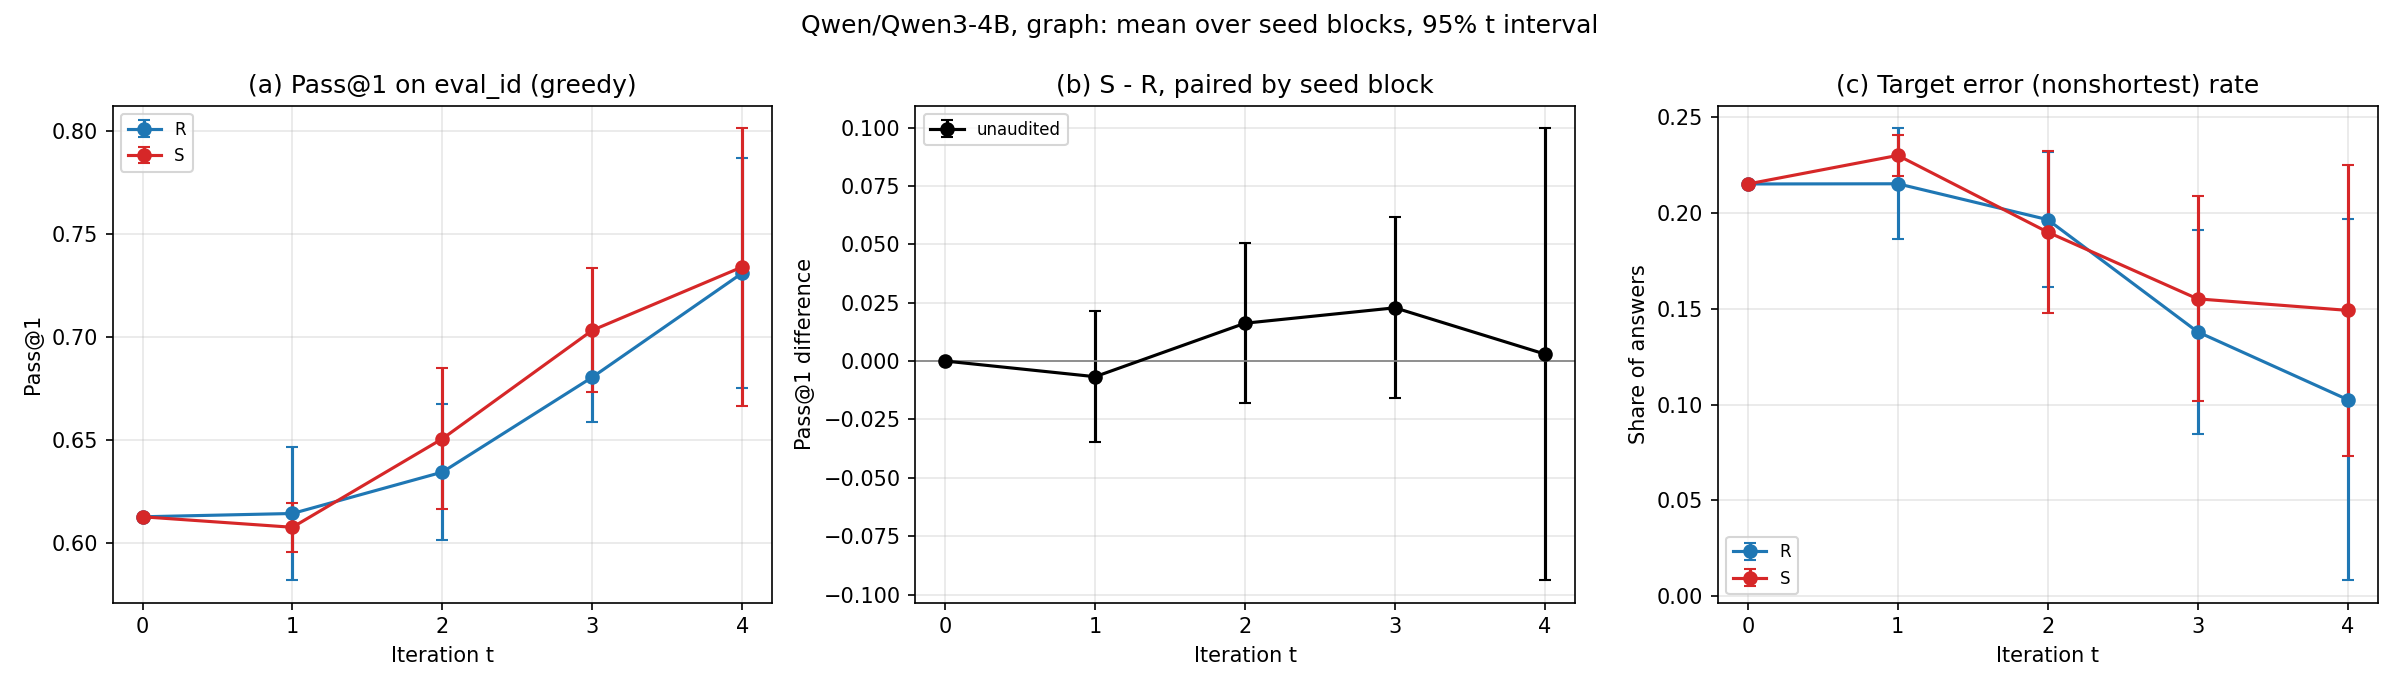
\includegraphics[width=0.90\linewidth]{figures/qwen4b_four_round_raw/unaudited_eval_id_pass1.png}
\par\smallskip
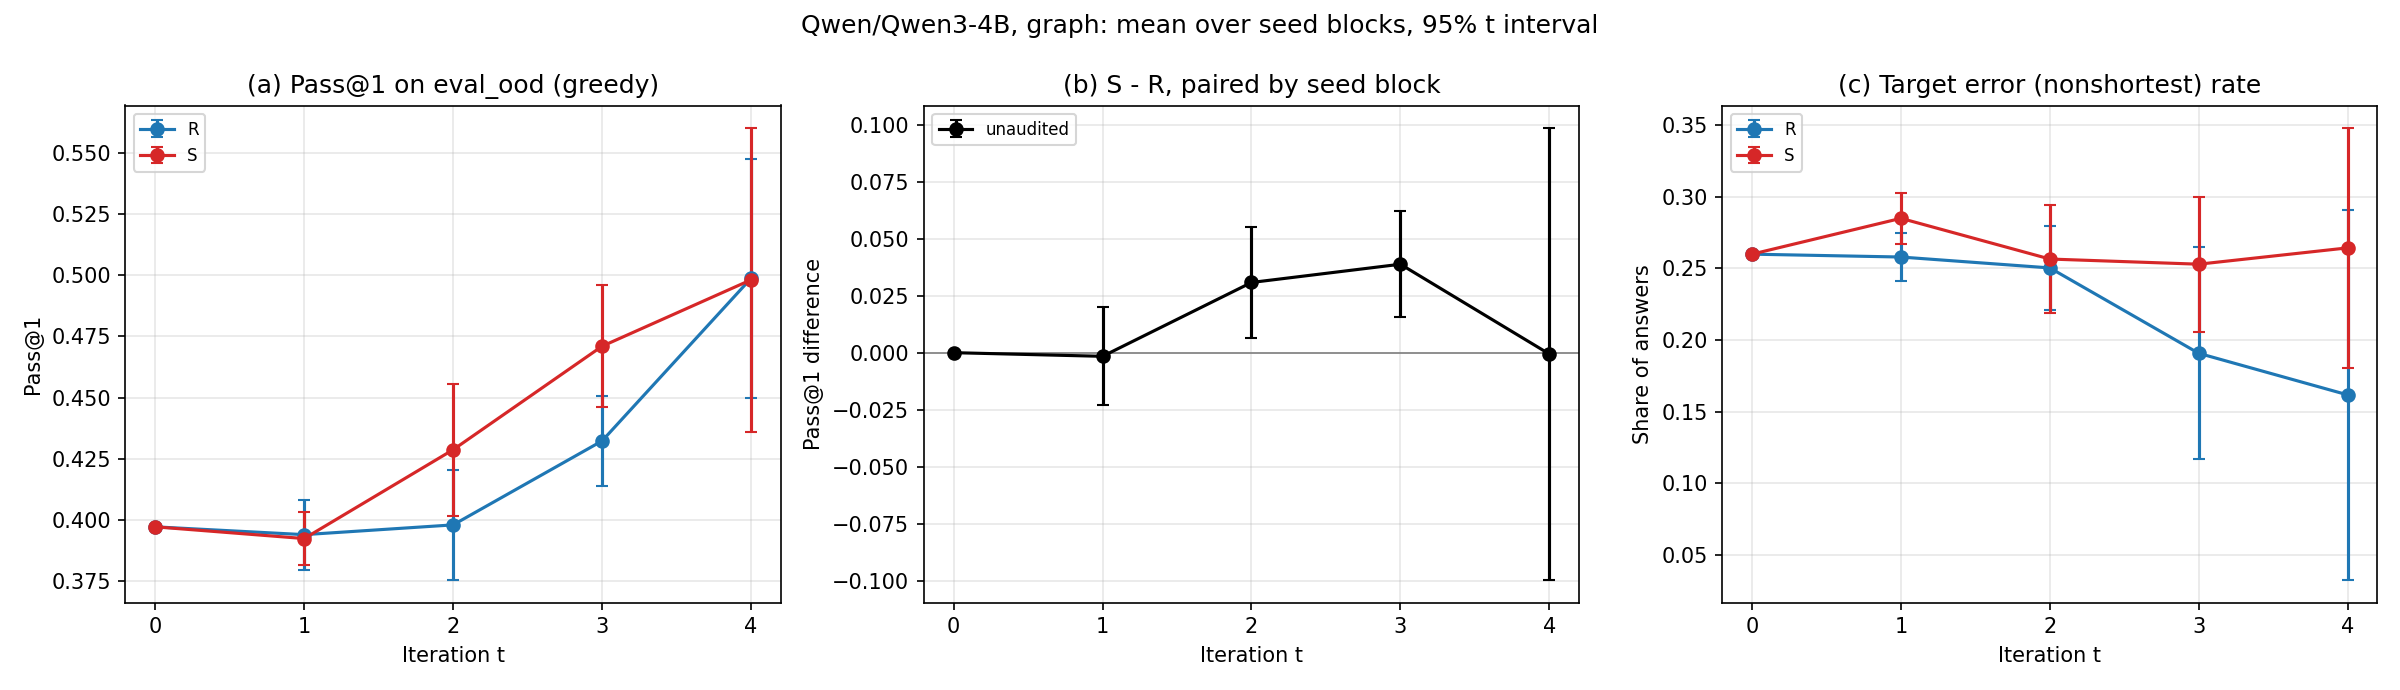
\includegraphics[width=0.90\linewidth]{figures/qwen4b_four_round_raw/unaudited_eval_ood_pass1.png}
\caption{Original unaudited Qwen3-4B graph curves, ID (top) and OOD
(bottom), for rounds 0--4. The panels show greedy Pass@1, paired
$S-R$ accuracy, and nonshortest-error incidence among all answers.}
\label{fig:qwen4b-raw-unaudited}
\end{figure}

Unaudited $R/S$ accuracy reaches $0.7309/0.7339$ ID and
$0.4988/0.4982$ OOD, from bases $0.6125$ and $0.3970$.
Paired endpoint contrasts are $0.0030\pm0.0968$ ID and
$-0.0006\pm0.0991$ OOD. The positive mean OOD contrast in
intermediate rounds declines to near zero at the endpoint.

\begin{figure}[H]
\centering
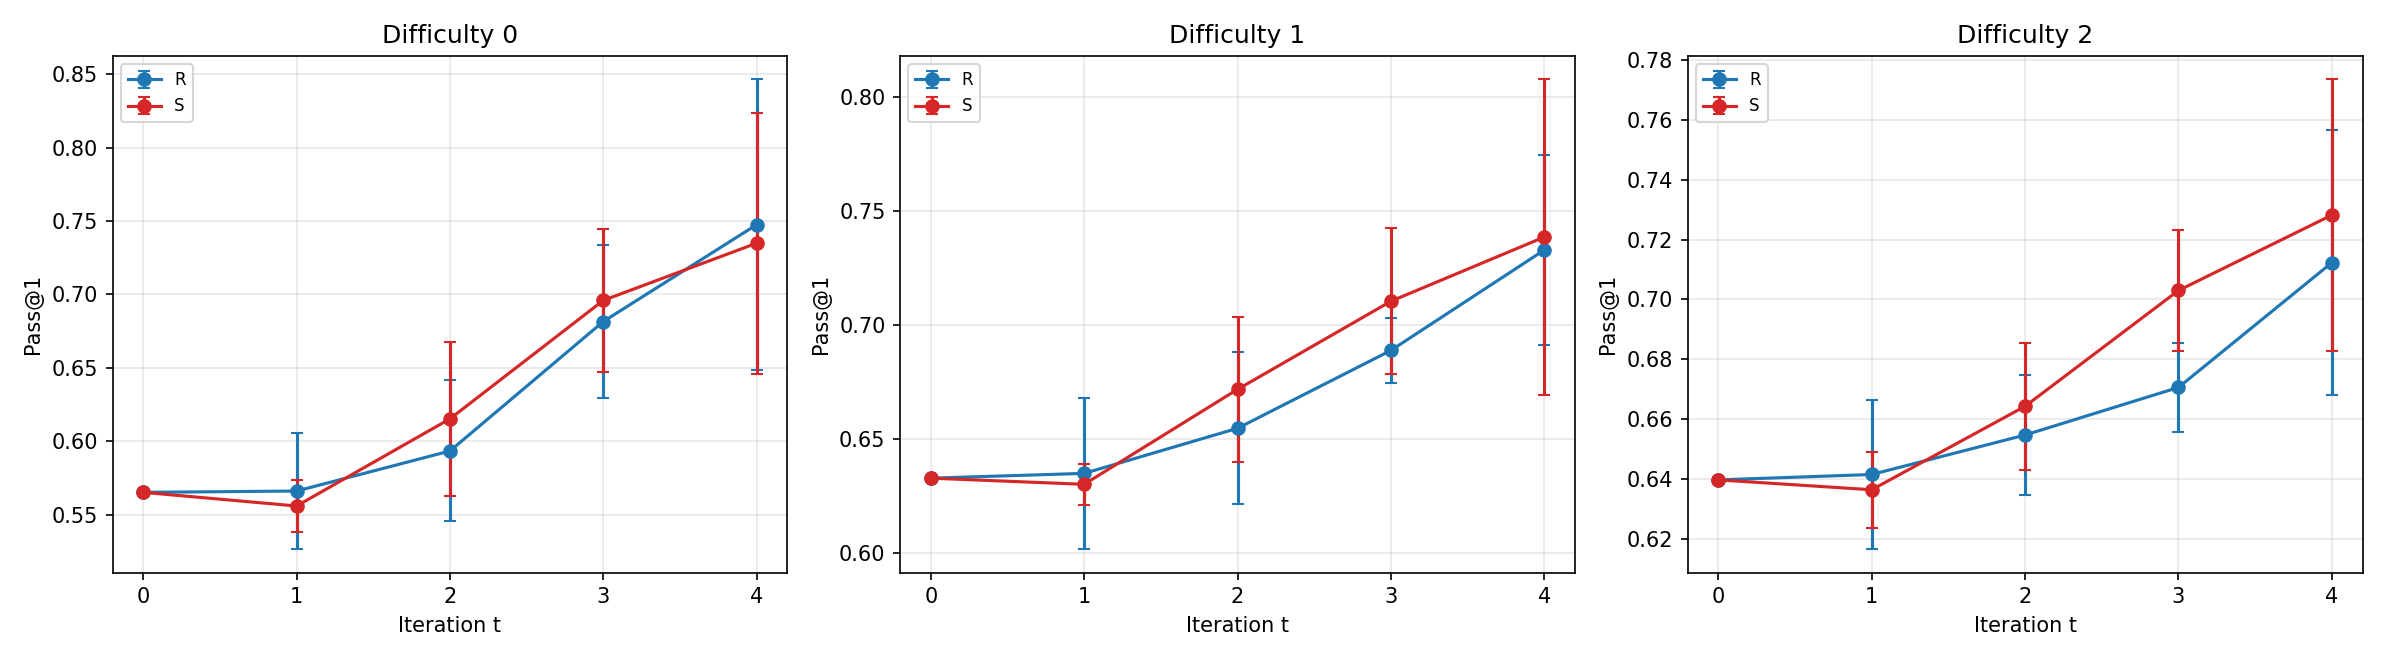
\includegraphics[width=0.90\linewidth]{figures/qwen4b_four_round_raw/unaudited_eval_id_by_difficulty.png}
\par\smallskip
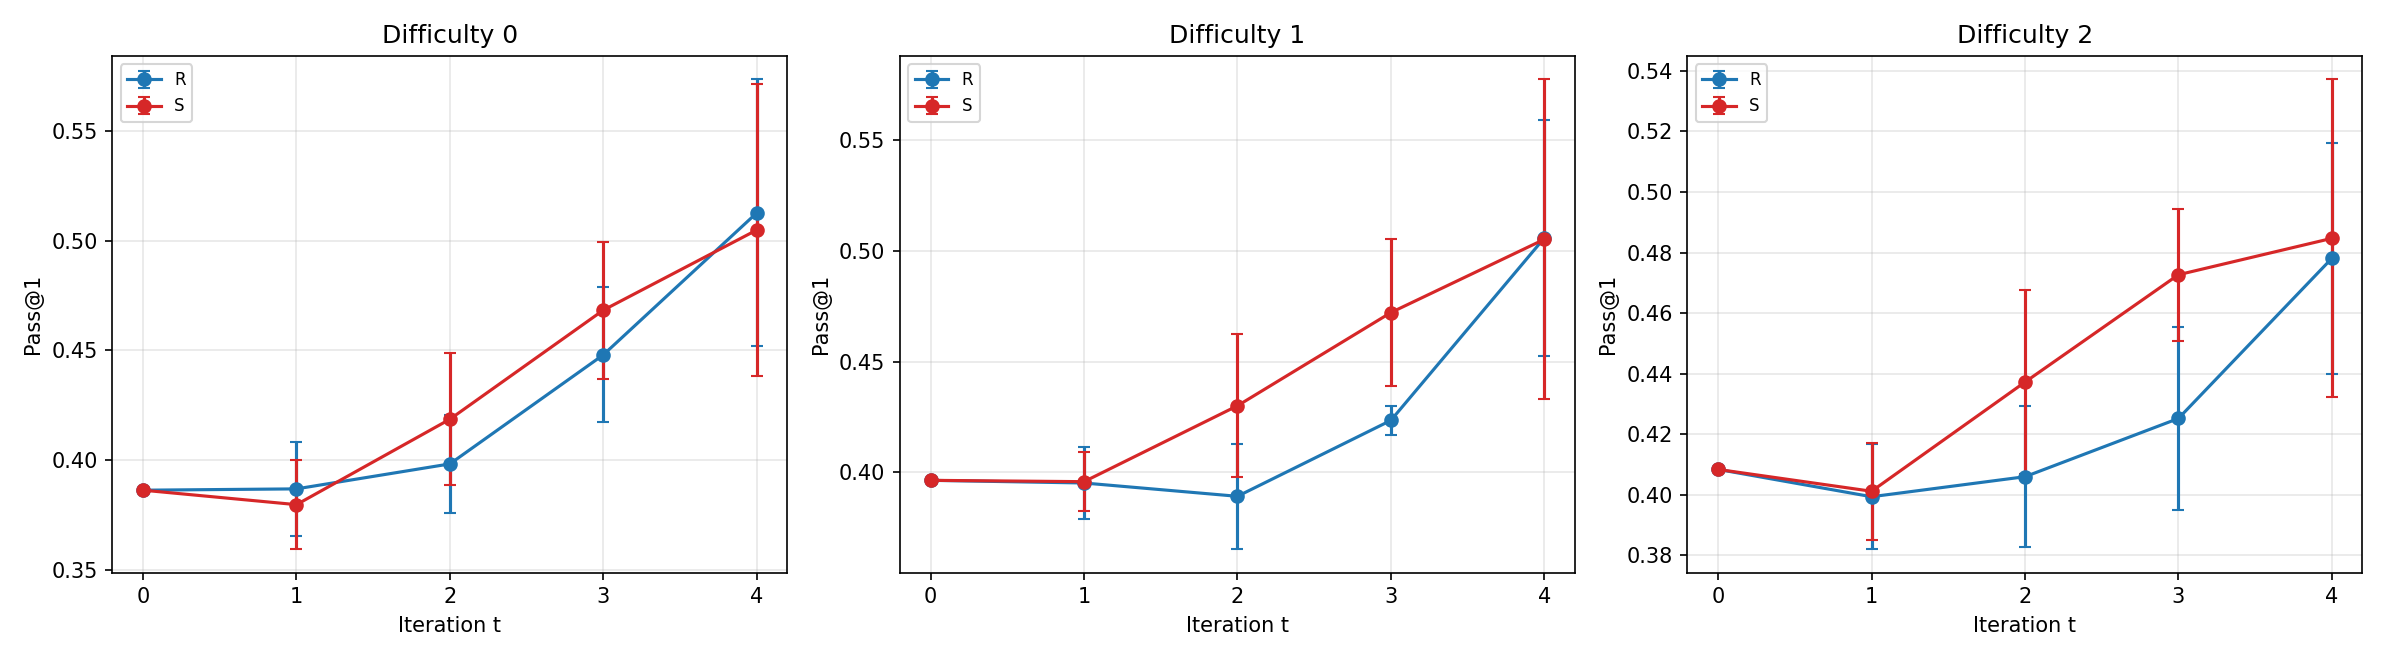
\includegraphics[width=0.90\linewidth]{figures/qwen4b_four_round_raw/unaudited_eval_ood_by_difficulty.png}
\caption{Original unaudited Qwen3-4B graph accuracy by generator
difficulty stratum, ID (top) and OOD (bottom), for rounds 0--4.
Strata 0--2 appear from left to right, containing $667/667/666$ ID
and $334/333/333$ OOD questions. Intervals use the same five blocks
as Figure~\ref{fig:qwen4b-raw-unaudited}.}
\label{fig:qwen4b-raw-unaudited-difficulty}
\end{figure}

The fixed generator strata do not establish a model-difficulty ordering.
Panel-specific vertical scales are retained, and these comparisons are
descriptive rather than multiplicity-adjusted. The breakdown provides
context for the aggregate trajectory without adding a stratum-level
accuracy claim.

\begin{figure}[H]
\centering
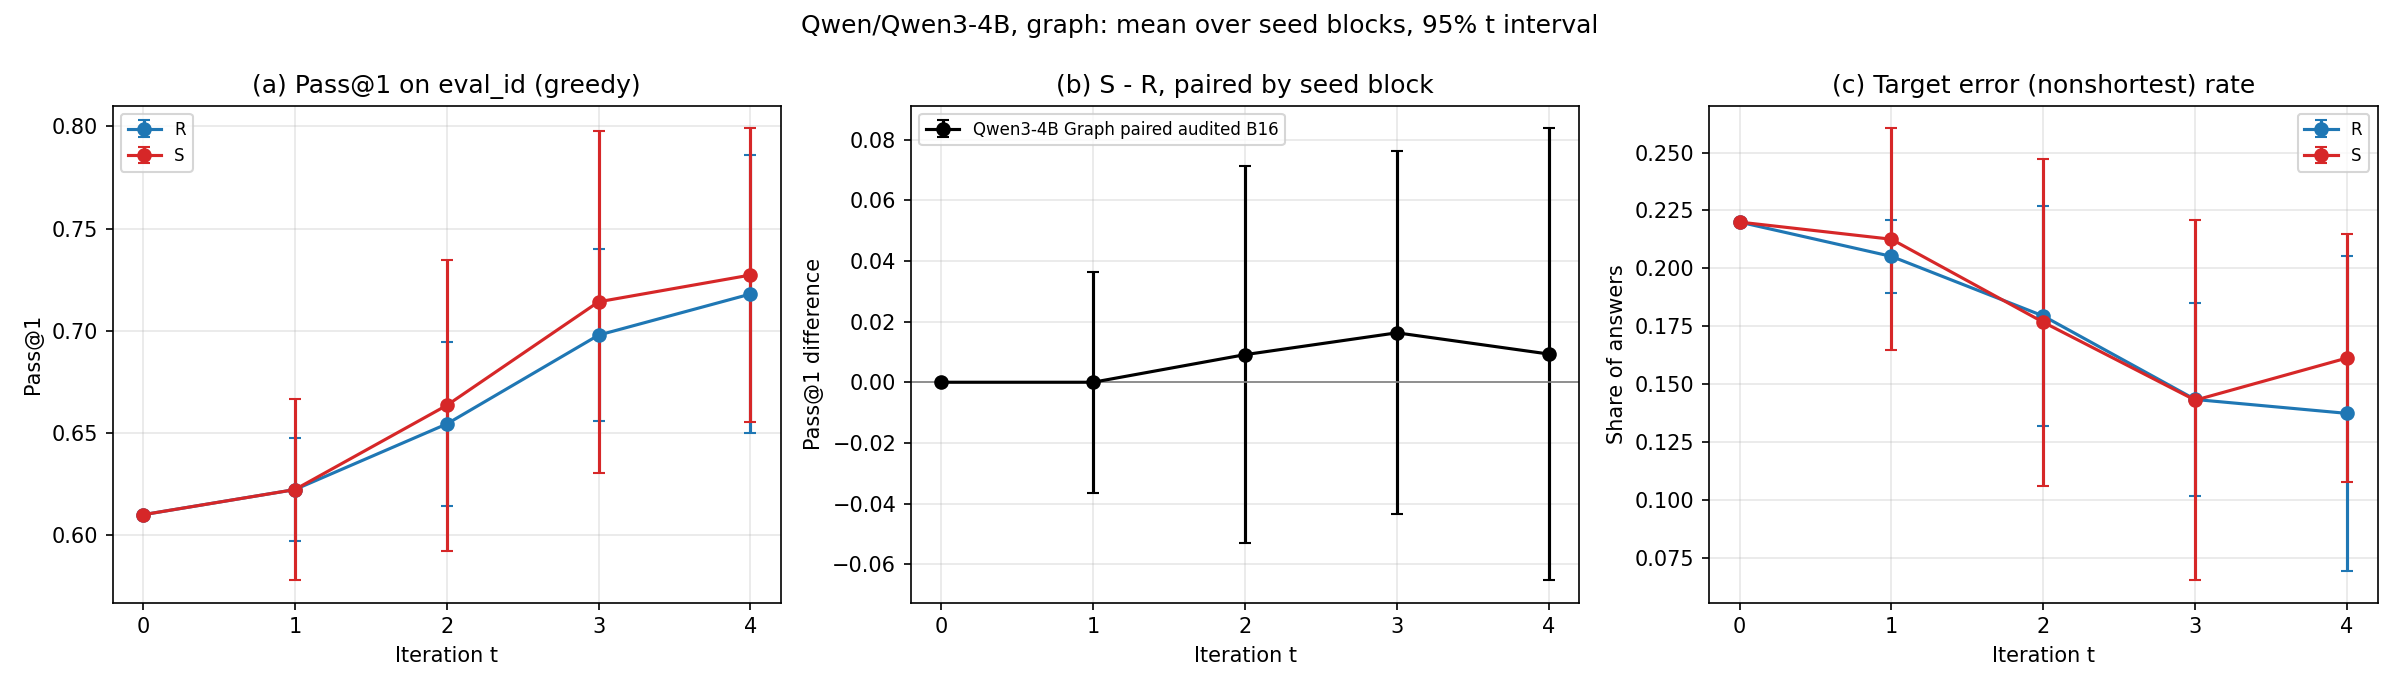
\includegraphics[width=0.90\linewidth]{figures/qwen4b_four_round_raw/audited_eval_id_pass1.png}
\par\smallskip
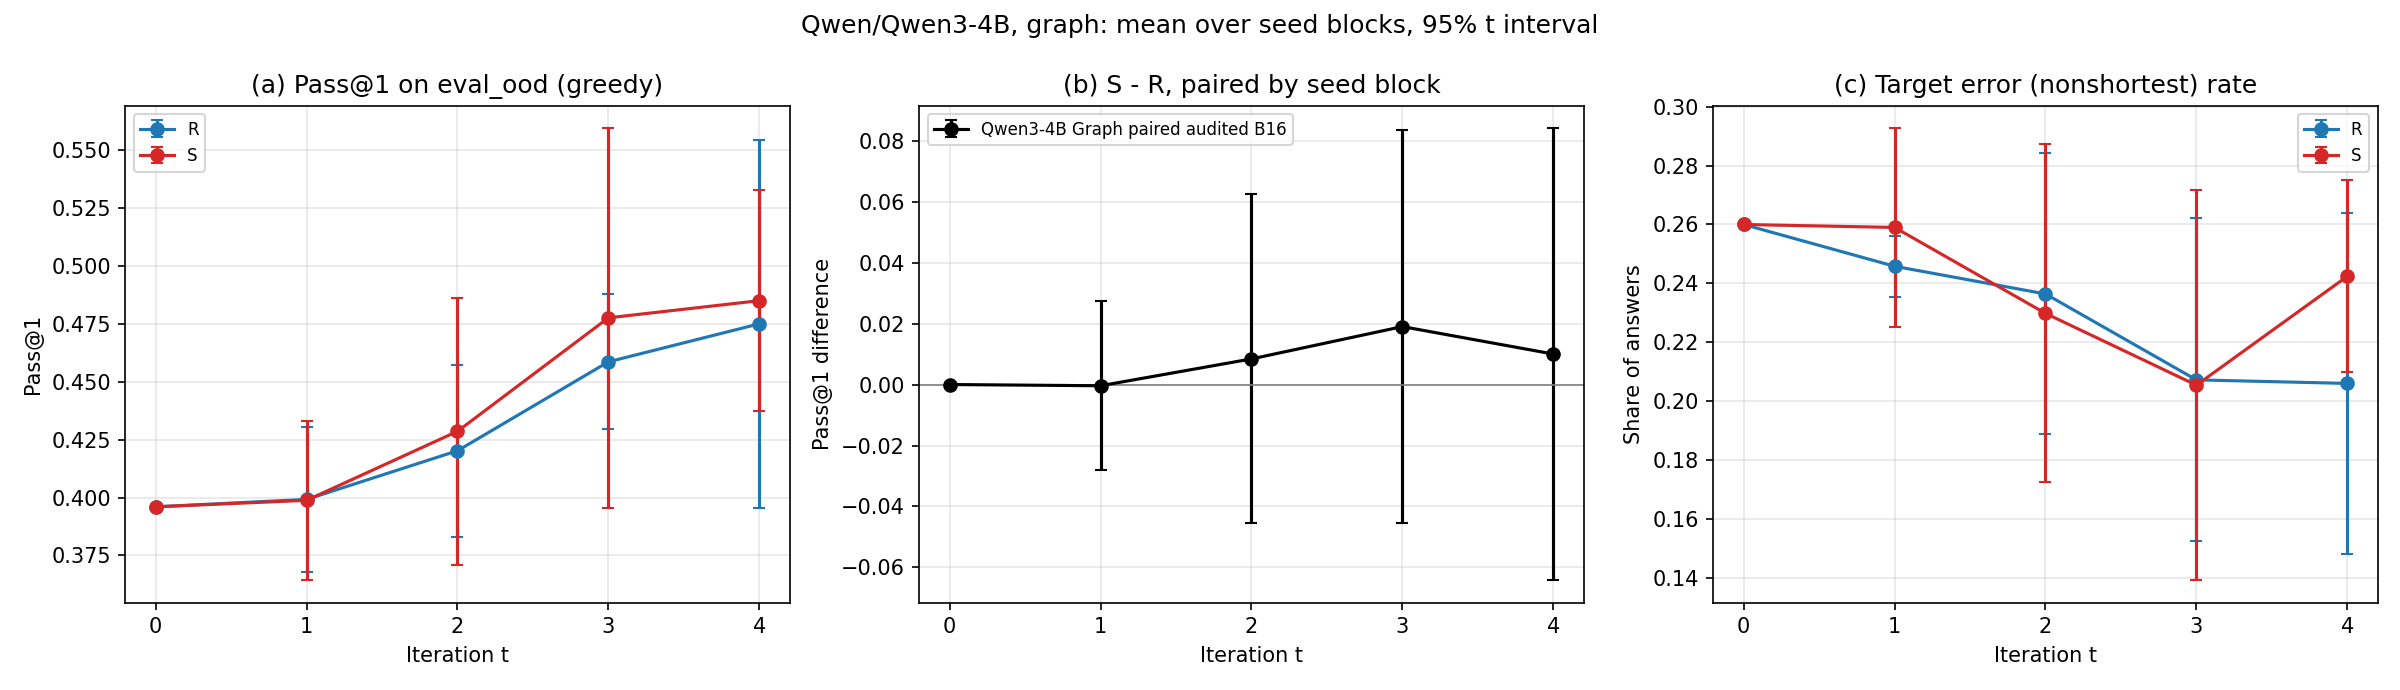
\includegraphics[width=0.90\linewidth]{figures/qwen4b_four_round_raw/audited_eval_ood_pass1.png}
\caption{Original adaptive-audit Qwen3-4B graph curves, ID (top)
and OOD (bottom), with 16 correctness queries per arm-round.
The panels show greedy Pass@1, paired $S-R$ accuracy, and
nonshortest-error incidence. Each audited arm spends 64 queries
over four rounds.}
\label{fig:qwen4b-raw-audited}
\end{figure}

Audited round-four $R/S$ accuracy is $0.7180/0.7273$ ID and
$0.4750/0.4850$ OOD, from audited-run bases $0.6100$ and $0.3960$.
The paired contrasts are $0.0093\pm0.0745$ and $0.0100\pm0.0741$.
They compare arms within the audited policy and
should not be interpreted as effects of auditing.

\begin{figure}[H]
\centering
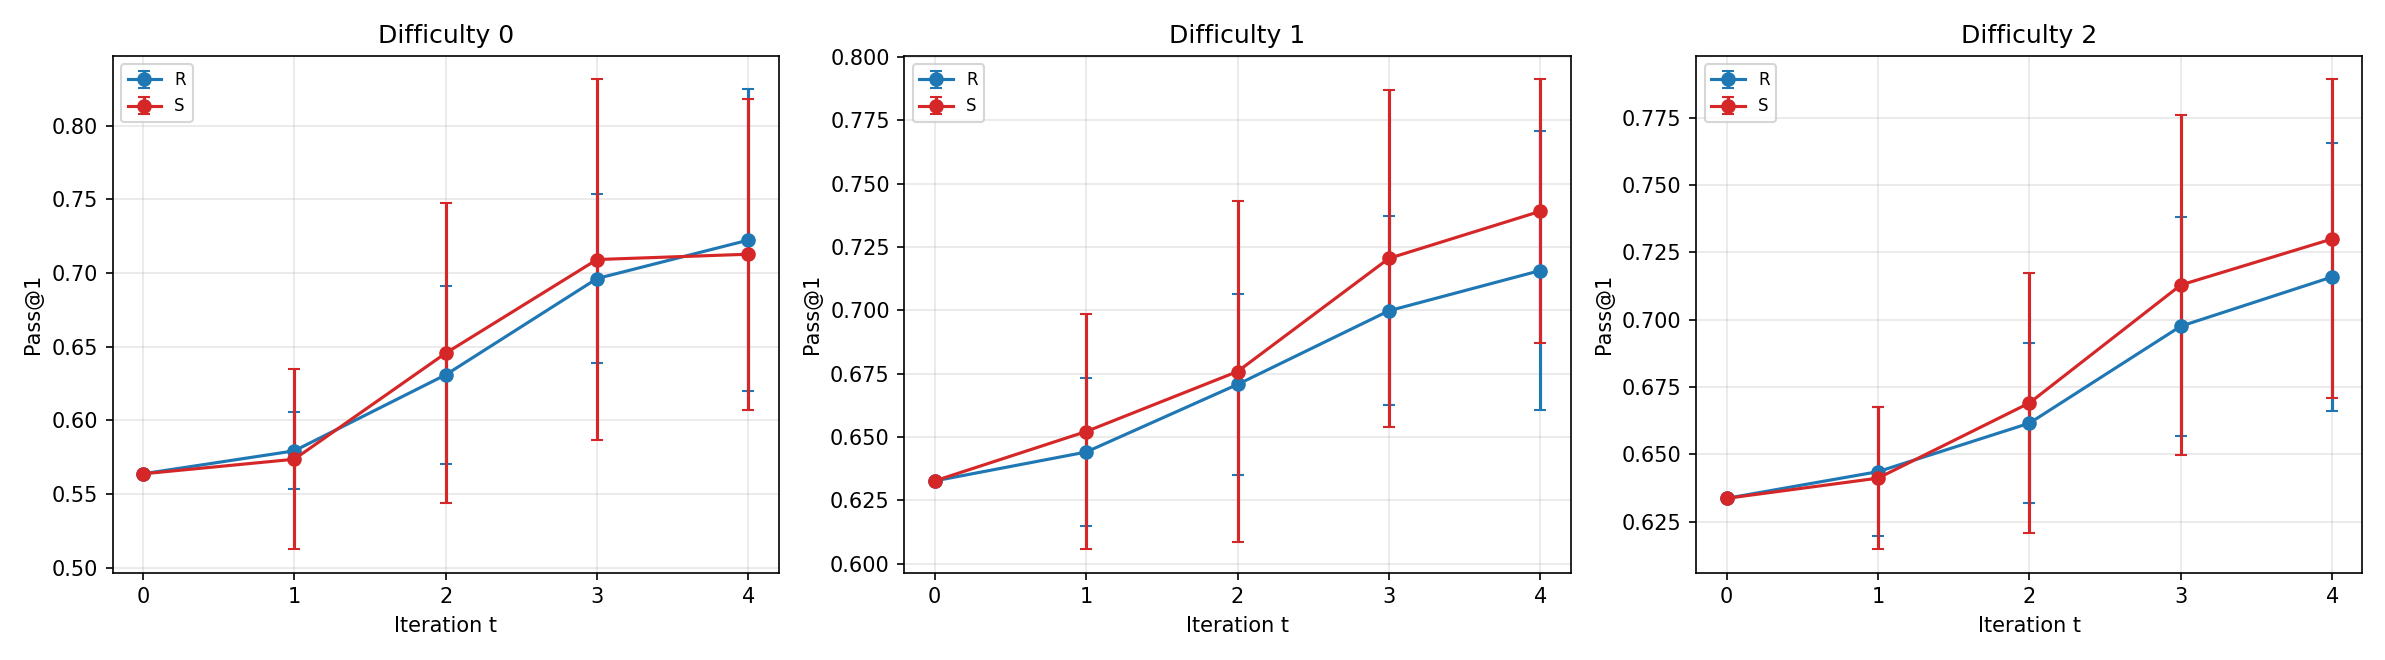
\includegraphics[width=0.90\linewidth]{figures/qwen4b_four_round_raw/audited_eval_id_by_difficulty.png}
\par\smallskip
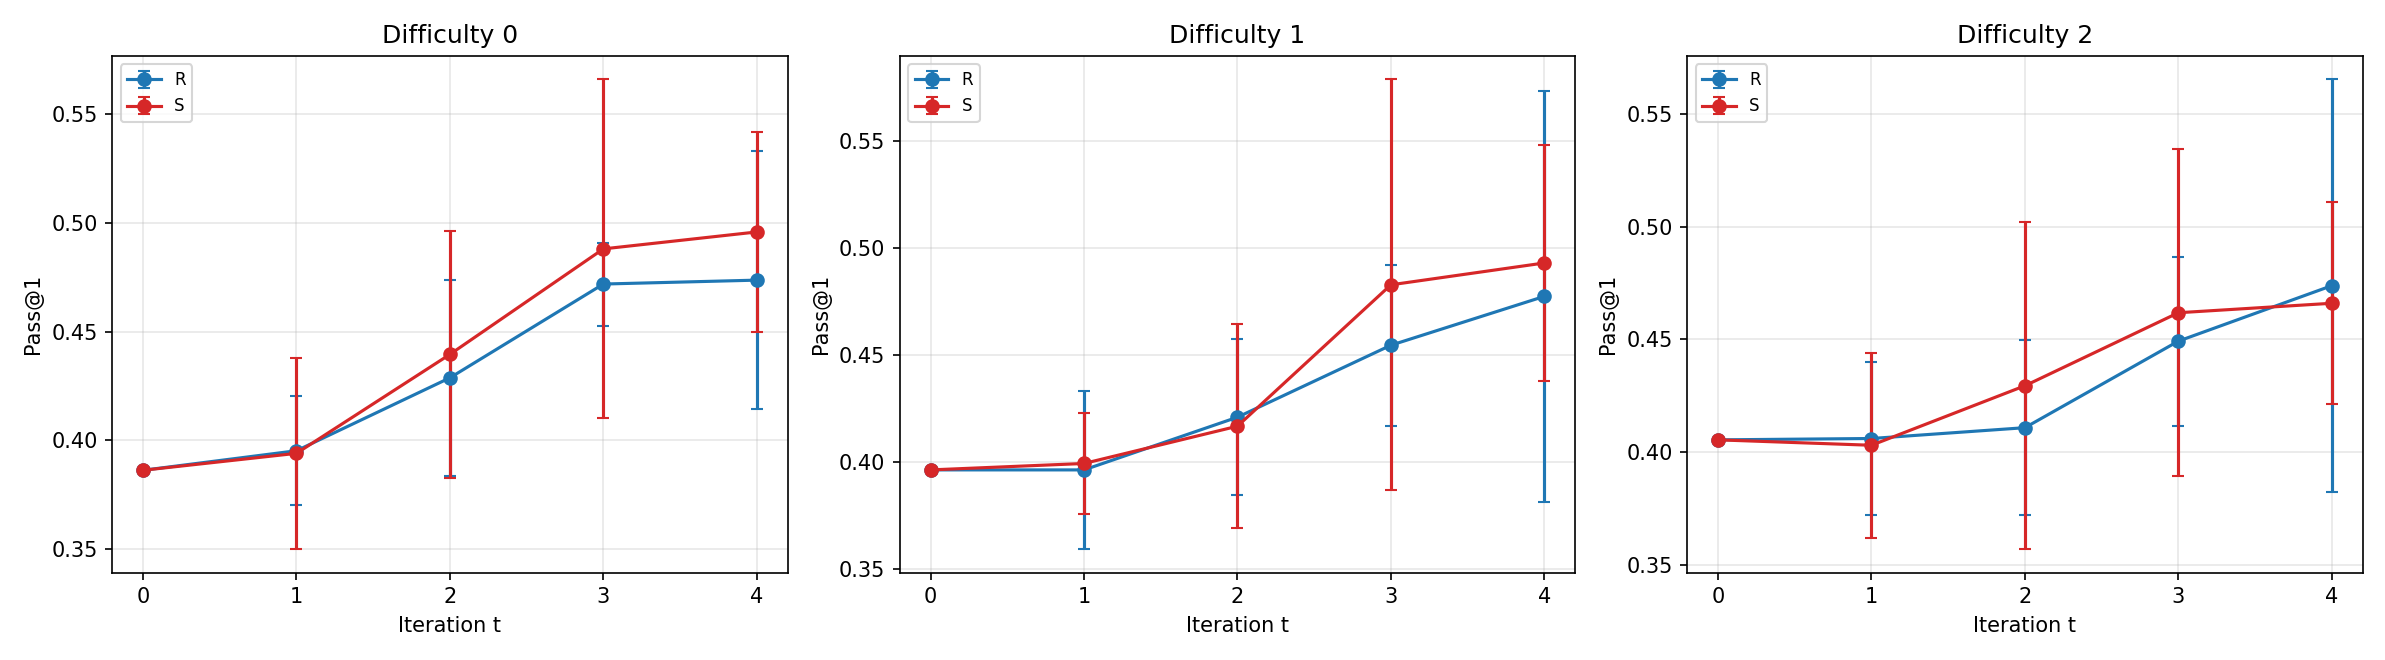
\includegraphics[width=0.90\linewidth]{figures/qwen4b_four_round_raw/audited_eval_ood_by_difficulty.png}
\caption{Original adaptive-audit Qwen3-4B graph accuracy by
generator stratum, ID (top) and OOD (bottom), for rounds 0--4.
Strata, fixed question sets, and interval conventions follow
Figure~\ref{fig:qwen4b-raw-unaudited-difficulty}.}
\label{fig:qwen4b-raw-audited-difficulty}
\end{figure}

The audited stratum curves use the same fixed questions and retain their
original panel-specific scales. They supplement the aggregate audited
results without establishing a stratum-specific audit benefit, which
would require a corresponding cross-policy comparison and treatment
of the multiple contrasts.

\begin{figure}[H]
\centering
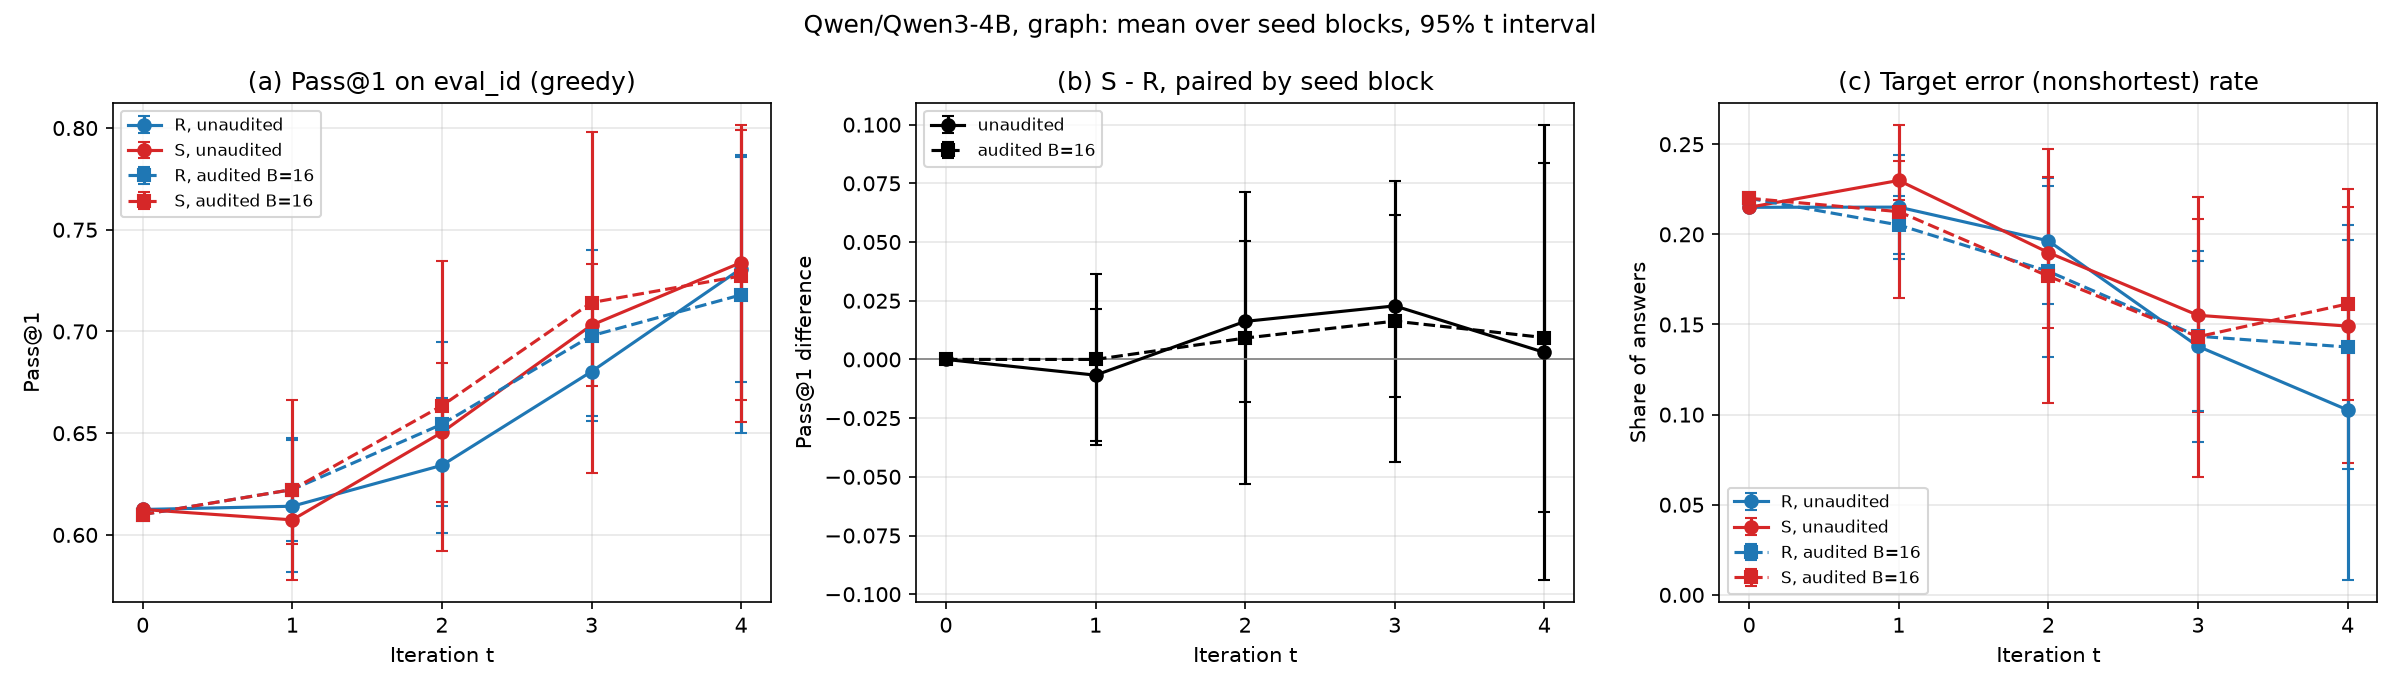
\includegraphics[width=0.90\linewidth]{figures/qwen4b_four_round_raw/comparison_eval_id_pass1.png}
\par\smallskip
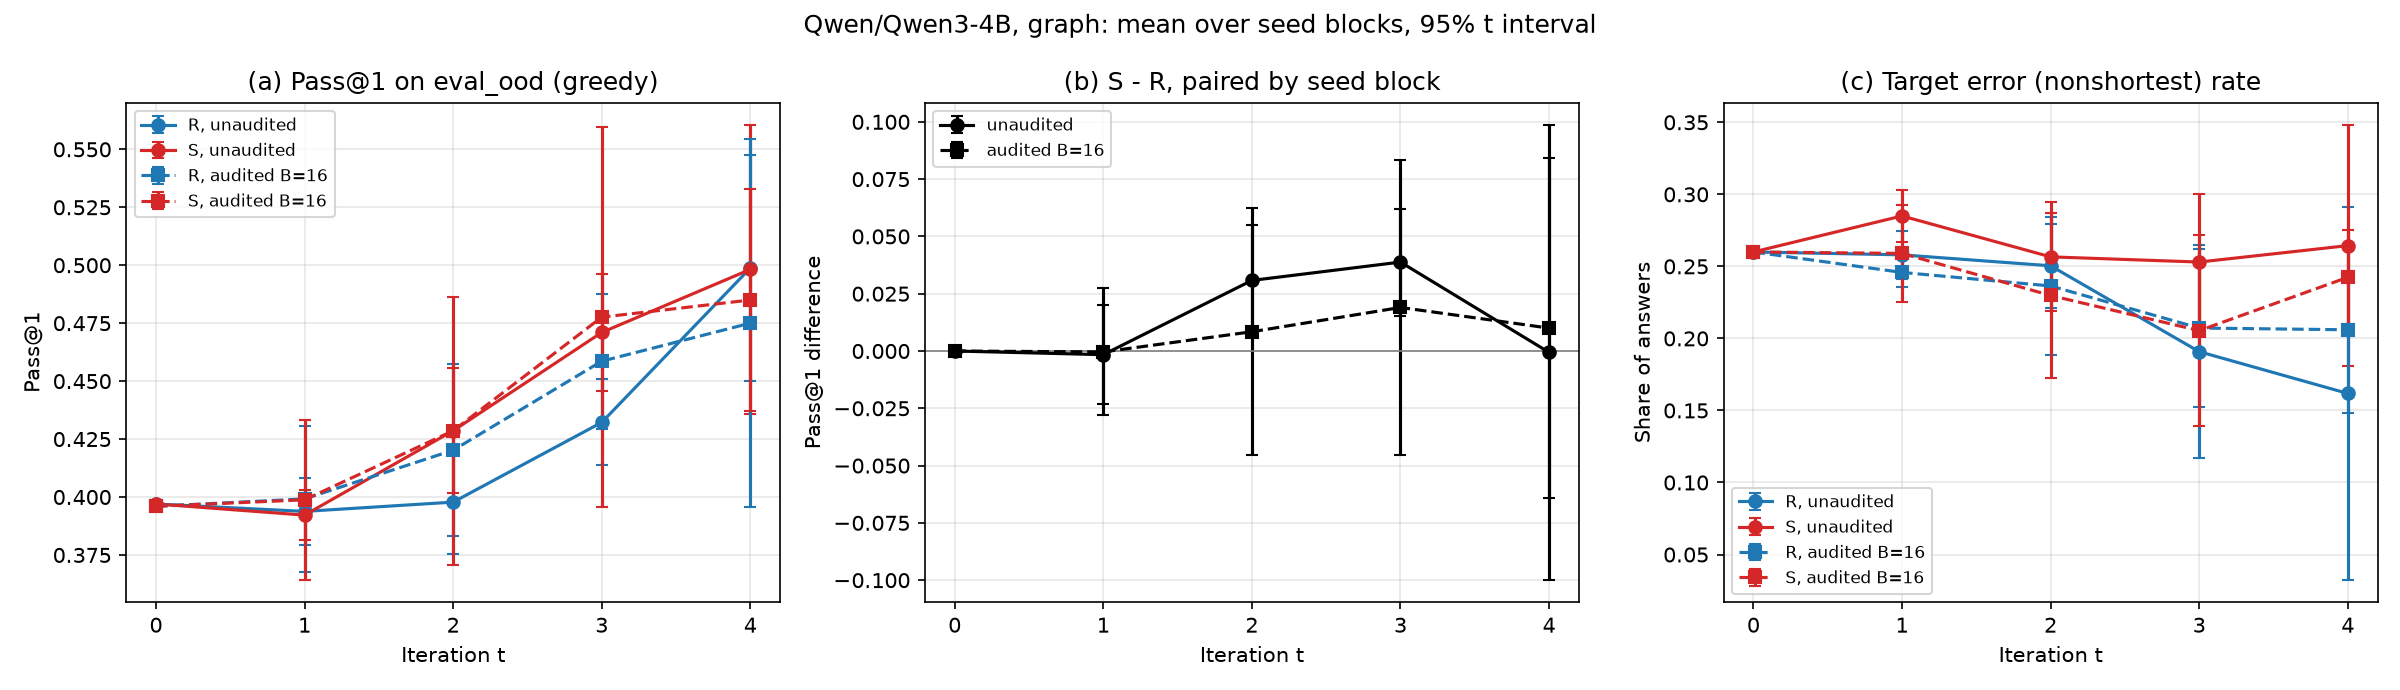
\includegraphics[width=0.90\linewidth]{figures/qwen4b_four_round_raw/comparison_eval_ood_pass1.png}
\caption{Joint Qwen3-4B graph trajectories, ID (top) and OOD
(bottom), generated with the original plotting method from the
same unaudited and audited checkpoints. The middle panels show
paired $S-R$ accuracy within each policy, not audited-minus-unaudited
effects.}
\label{fig:qwen4b-raw-comparison}
\end{figure}

Same-arm audit error changes are positive in mean
(Table~\ref{tab:audit-results}). Differences in optimizer effort
limit causal attribution: these results establish
neither an audit benefit nor a detrimental audit effect.

\begin{figure}[H]
\centering
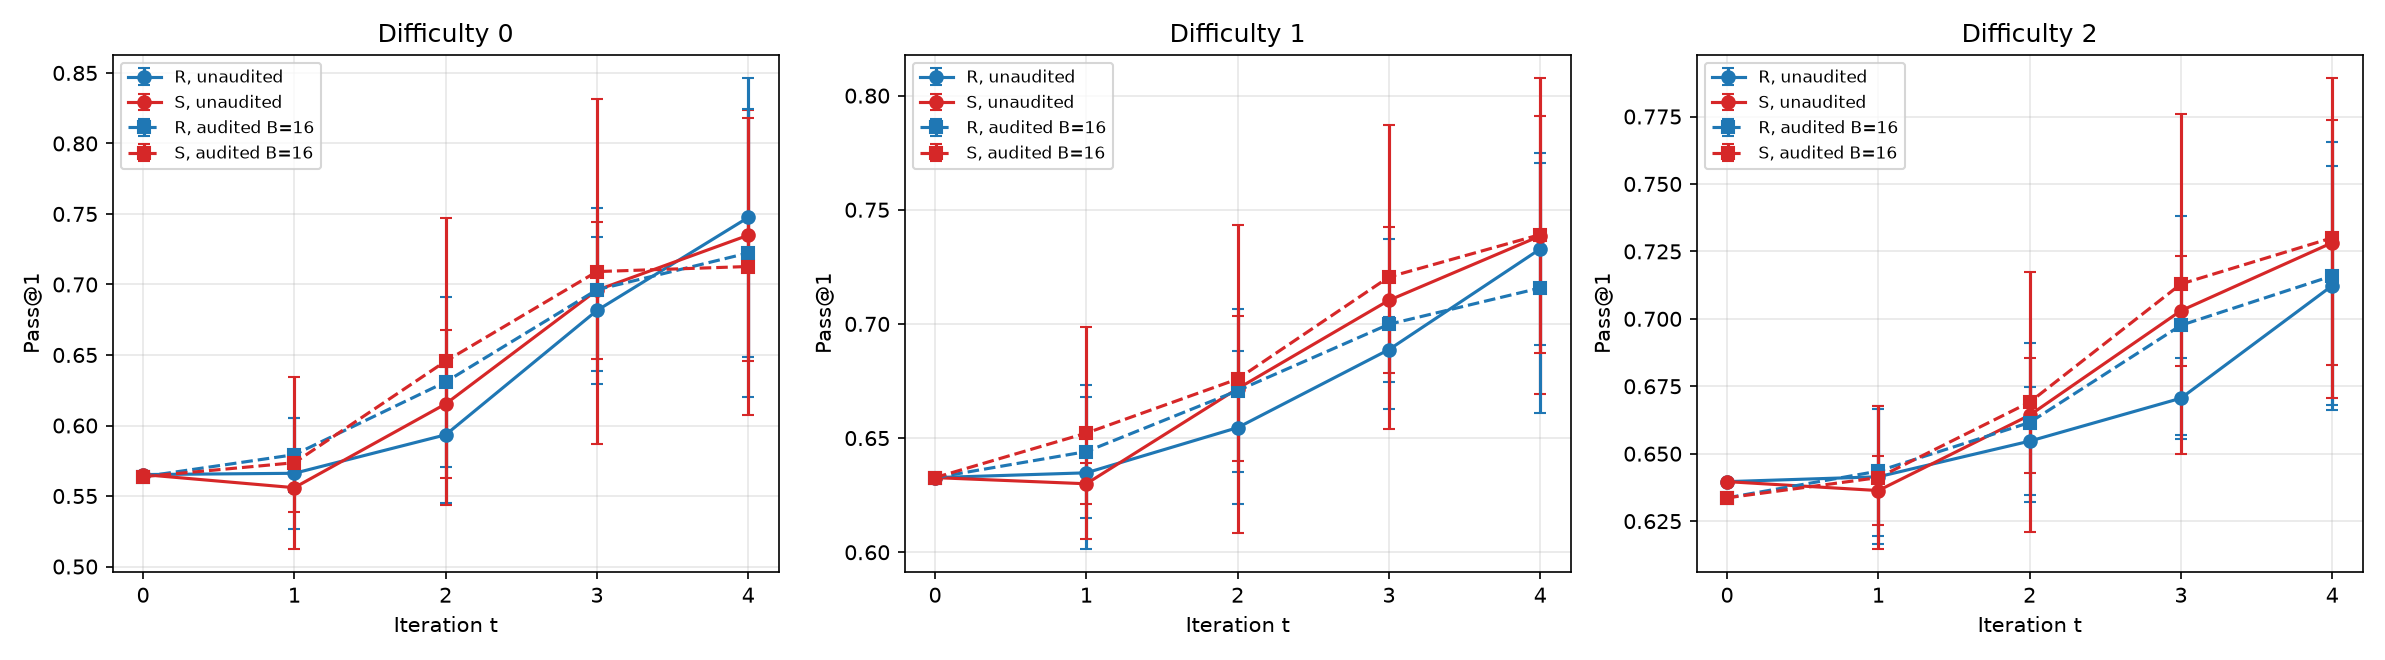
\includegraphics[width=0.90\linewidth]{figures/qwen4b_four_round_raw/comparison_eval_id_by_difficulty.png}
\par\smallskip
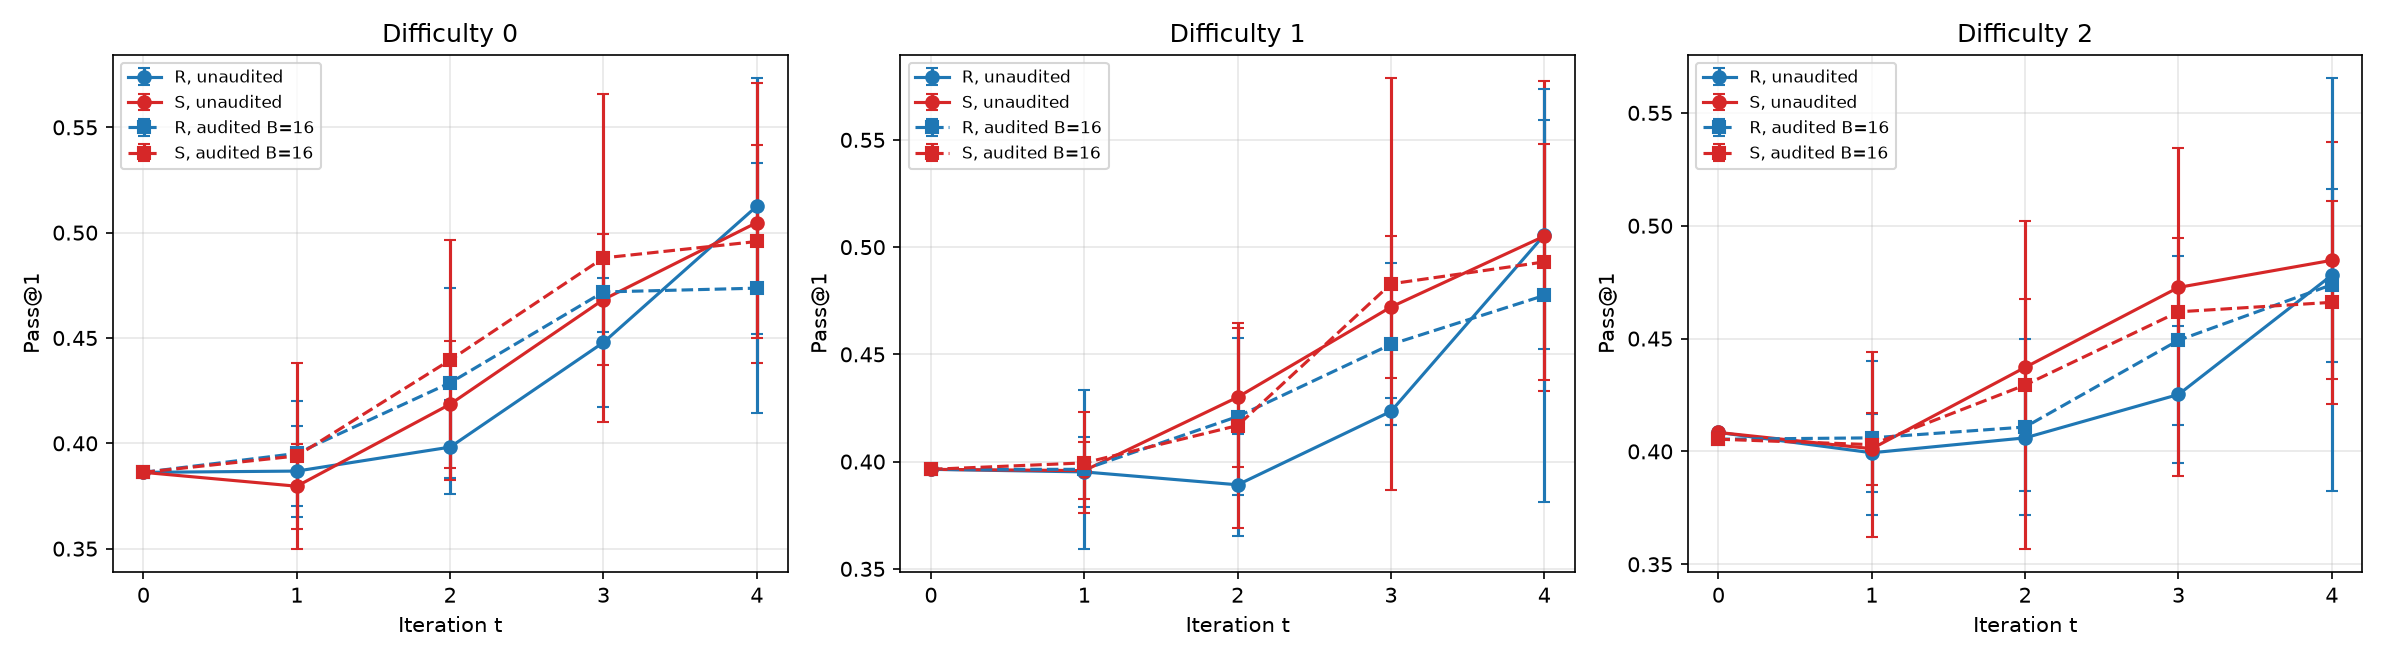
\includegraphics[width=0.90\linewidth]{figures/qwen4b_four_round_raw/comparison_eval_ood_by_difficulty.png}
\caption{Joint Qwen3-4B graph accuracy by generator stratum, ID
(top) and OOD (bottom), generated from the same checkpoint records
with the original plotting method. Both policies and arms use the
same question stratum at each checkpoint. Counts and interval
conventions follow Figure~\ref{fig:qwen4b-raw-unaudited-difficulty}.}
\label{fig:qwen4b-raw-comparison-difficulty}
\end{figure}

The two policies and arms share each question stratum. Panel-specific vertical scales are
unchanged, and the intervals are not adjusted across strata, rounds,
or policies. Consequently the joint breakdown remains descriptive,
consistent with the aggregate uncertainty rather than a separate
confirmatory analysis.
\endgroup

